\documentclass[journal,12pt,twocolumn]{IEEEtran}
\usepackage{amsthm}
\allowbreak
\usepackage{setspace}
\usepackage{gensymb}
\singlespacing
\usepackage[cmex10]{amsmath}
\usepackage{caption}
\usepackage{amsthm}



\DeclareUnicodeCharacter{2212}{-}
\usepackage{tikz}
\usepackage{pgfplots}
\usepackage{tkz-fct}
\usepackage{mathrsfs}
\usepackage{txfonts}
\usepackage{stfloats}
\usepackage{bm}
\usepackage{cite}
\usepackage{cases}
\usepackage{subfig}

\usepackage{longtable}
\usepackage{multirow}

\usepackage{enumitem}
\usepackage{mathtools}
\usepackage{steinmetz}
\usepackage{tikz}
\usepackage{circuitikz}
\usepackage{verbatim}
\usepackage{tfrupee}
\usepackage[breaklinks=true]{hyperref}
\usepackage{graphicx}
\usepackage{tkz-euclide}
\graphicspath{ {./images/} }
\usetikzlibrary{calc,math}
\usepackage{listings}
    \usepackage{color}                                            %%
    \usepackage{array}                                            %%
    \usepackage{longtable}                                        %%
    \usepackage{calc}                                             %%
    \usepackage{multirow}                                         %%
    \usepackage{hhline}                                           %%
    \usepackage{ifthen}                                           %%
    \usepackage{lscape}     
\usepackage{multicol}
\usepackage{chngcntr}

\DeclareMathOperator*{\Res}{Res}

\renewcommand\thesection{\arabic{section}}
\renewcommand\thesubsection{\thesection.\arabic{subsection}}
\renewcommand\thesubsubsection{\thesubsection.\arabic{subsubsection}}

\renewcommand\thesectiondis{\arabic{section}}
\renewcommand\thesubsectiondis{\thesectiondis.\arabic{subsection}}
\renewcommand\thesubsubsectiondis{\thesubsectiondis.\arabic{subsubsection}}


\hyphenation{op-tical net-works semi-conduc-tor}
\def\inputGnumericTable{}                                 %%

\lstset{
%language=C,
frame=single, 
breaklines=true,
columns=fullflexible
}
\begin{document}


\newtheorem{theorem}{Theorem}[section]
\newtheorem{problem}{Problem}
\newtheorem{proposition}{Proposition}[section]
\newtheorem{lemma}{Lemma}[section]
\newtheorem{corollary}[theorem]{Corollary}
\newtheorem{example}{Example}[section]
\newtheorem{definition}[problem]{Definition}

\newcommand{\BEQA}{\begin{eqnarray}}
\newcommand{\EEQA}{\end{eqnarray}}
\newcommand{\define}{\stackrel{\triangle}{=}}
\bibliographystyle{IEEEtran}
\raggedbottom
\setlength{\parindent}{0pt}
\providecommand{\mbf}{\mathbf}
\providecommand{\pr}[1]{\ensuremath{\Pr\left(#1\right)}}
\providecommand{\qfunc}[1]{\ensuremath{Q\left(#1\right)}}
\providecommand{\sbrak}[1]{\ensuremath{{}\left[#1\right]}}
\providecommand{\lsbrak}[1]{\ensuremath{{}\left[#1\right.}}
\providecommand{\rsbrak}[1]{\ensuremath{{}\left.#1\right]}}
\providecommand{\brak}[1]{\ensuremath{\left(#1\right)}}
\providecommand{\lbrak}[1]{\ensuremath{\left(#1\right.}}
\providecommand{\rbrak}[1]{\ensuremath{\left.#1\right)}}
\providecommand{\cbrak}[1]{\ensuremath{\left\{#1\right\}}}
\providecommand{\lcbrak}[1]{\ensuremath{\left\{#1\right.}}
\providecommand{\rcbrak}[1]{\ensuremath{\left.#1\right\}}}
\theoremstyle{remark}
\newtheorem{rem}{Remark}
\newcommand{\sgn}{\mathop{\mathrm{sgn}}}
\providecommand{\abs}[1]{$\left\vert#1\right\vert$}
\providecommand{\res}[1]{\Res\displaylimits_{#1}} 
\providecommand{\norm}[1]{$\left\lVert#1\right\rVert$}
%\providecommand{\norm}[1]{\lVert#1\rVert}
\providecommand{\mtx}[1]{\mathbf{#1}}
\providecommand{\mean}[1]{E$\left[ #1 \right]$}
\providecommand{\fourier}{\overset{\mathcal{F}}{ \rightleftharpoons}}
%\providecommand{\hilbert}{\overset{\mathcal{H}}{ \rightleftharpoons}}
\providecommand{\system}{\overset{\mathcal{H}}{ \longleftrightarrow}}
	%\newcommand{\solution}[2]{\textbf{Solution:}{#1}}
\newcommand{\solution}{\noindent \textbf{Solution: }}
\newcommand{\cosec}{\,\text{cosec}\,}
\providecommand{\dec}[2]{\ensuremath{\overset{#1}{\underset{#2}{\gtrless}}}}
\newcommand{\myvec}[1]{\ensuremath{\begin{pmatrix}#1\end{pmatrix}}}
\newcommand{\mydet}[1]{\ensuremath{\begin{vmatrix}#1\end{vmatrix}}}
\numberwithin{equation}{subsection}
\makeatletter
\@addtoreset{figure}{problem}
\makeatother
\let\StandardTheFigure\thefigure
\let\vec\mathbf
\renewcommand{\thefigure}{\theproblem}
\def\putbox#1#2#3{\makebox[0in][l]{\makebox[#1][l]{}\raisebox{\baselineskip}[0in][0in]{\raisebox{#2}[0in][0in]{#3}}}}
     \def\rightbox#1{\makebox[0in][r]{#1}}
     \def\centbox#1{\makebox[0in]{#1}}
     \def\topbox#1{\raisebox{-\baselineskip}[0in][0in]{#1}}
     \def\midbox#1{\raisebox{-0.5\baselineskip}[0in][0in]{#1}}
\vspace{3cm}
\title{AI1103: Challenge Problem Mixture}
\author{Tanmay Garg \\CS20BTECH11063 EE20BTECH11048}
\maketitle
\newpage
\bigskip
\renewcommand{\thefigure}{\theenumi}
\renewcommand{\thetable}{\theenumi}
%
Download all python codes from 
\begin{lstlisting}
https://github.com/tanmaygar/AI-Course/blob/main/challenge%20mixture/codes/challenge_mix.py
\end{lstlisting}
%
and latex-tikz codes from 
%
\begin{lstlisting}
https://github.com/tanmaygar/AI-Course/blob/main/challenge%20mixture/Challenge_Mixed.tex
\end{lstlisting}
\section*{Challenge Problem Mixed}
Let $X \sim B\brak{5,\frac{1}{2}}$ and $Y \sim U(0,1)$. The the value of:
\[
    \frac{\pr{X+Y \leq 2}}{\pr{X+Y \geq 5}}
\]
is equal to? ($X$ and $Y$ are independent)
\section*{Solution: Characteristic function approach}
Characteristic function for $X \sim B\brak{5,\frac{1}{2}}$ will be:
\begin{align}
    C_X(t)=\brak{\frac{e^{it}+1}{2}}^5
\end{align}
Characteristic function for $Y \sim U(0,1)$ will be:
\begin{align}
    C_Y(t)=\frac{e^{it}-1}{it}
\end{align}
Since both $X$ and $Y$ are independent we can take:
\begin{align}
    Z&=X+Y\\
    C_Z(t)&=C_X(t)C_Y(t)\\
    C_Z(t)&= \frac{(e^{it}+1)^5(e^{it}-1)}{32it}
\end{align}
Applying Gil-Pelaez formula:
\begin{align}
    F_Z(z)=\frac{1}{2}-\frac{1}{\pi}\int_0^\infty \frac{\text{Im}\brak{e^{-itz}C_Z(t)}}{t}dt
\end{align}
\begin{multline*}
    F_Z(z)=\frac{1}{2}-\frac{1}{\pi}\int_0^\infty\frac{1}{2it}\brak{\frac{(e^{it}+1)^5(e^{it}-1)e^{-itz}}{32it}}\\+\frac{1}{2it}\brak{\frac{(e^{-it}+1)^5(e^{-it}-1)e^{itz}}{32it}}dt
\end{multline*}
Substituting $z=2$, the value for $\pr{Z\leq 2}$:
\begin{align}
\nonumber
    &=\frac{1}{2}+\frac{1}{\pi}\int_0^\infty \frac{8\cos{2t}+2\cos{4t}}{64t^2}dt\\
    &\quad+\frac{1}{\pi}\int_0^\infty\frac{+8\cos{3t}-8\cos{t}-10}{64t^2}dt\\
    &=\frac{1}{2}+\frac{1}{\pi}\times\frac{-5\pi}{16}=\frac{3}{16}\label{first_value}
\end{align}
Similarly on substituting $z=5$, the value for $\pr{Z\leq 5}$:
\begin{align}
\nonumber
    &=\frac{1}{2} +\frac{1}{\pi}\int_0^\infty\frac{-10\cos{3t}-8\cos{4t}}{64t^2}dt\\&\quad +\frac{1}{\pi}\int_0^\infty\frac{-2\cos{5t}+12\cos{t}+8}{64t^2}dt\\
    &=\frac{1}{2}+\frac{1}{\pi}\times \frac{15\pi}{32}=\frac{31}{32}
\end{align}
The value for $\pr{Z\geq 5}$:
\begin{align}
    \pr{Z>5}&=1-\pr{Z\leq 5}\\
    &=1-\frac{31}{32}=\frac{1}{32}\label{second_value}
\end{align}
Upon substituting \eqref{first_value}and \eqref{second_value}, we get:
\begin{align}
    \frac{\pr{X+Y \leq 2}}{\pr{X+Y \geq 5}} = 6
\end{align}
\begin{figure}[h]
    \centering
    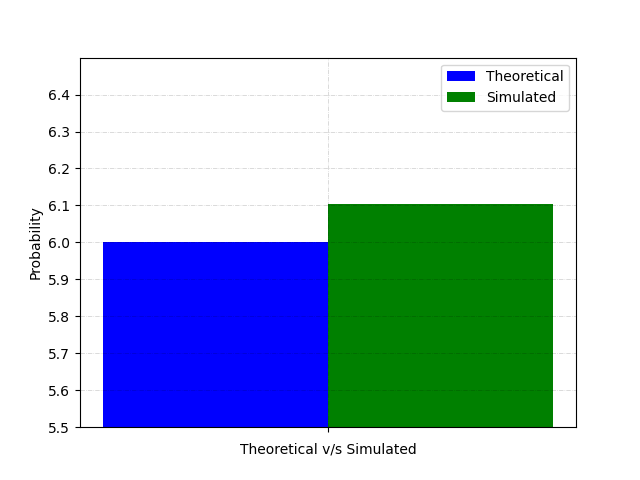
\includegraphics[width = 0.9\columnwidth]{Figure_1.png}
    \caption{}
    \label{fig:my_label}
\end{figure}
\end{document}